% =====================================================================
%  §1. Матрицы Джонса: язык поляризационной оптики
%
%  ЖАНР (STYLE.md): учебная литература. Ни путей, ни имён программ, ни
%  номеров гипотез. Прослеживаемость — ключи \srckey{1.x} и приложение.
%
%  Содержательная основа: primers/01_jones_polarization.md (markdown
%  первичен по фактуре, LaTeX — по подаче).
% =====================================================================
\section{Матрицы Джонса: язык поляризационной оптики}
\label{sec:jones}
\markboth{§\thesection. Матрицы Джонса}{}

В §\ref{sec:electrodynamics} решётка проводов свелась к двум комплексным числам на каждой частоте.
Теперь нужен аппарат, который позволит собрать из таких элементов \emph{установку} и получить
формулу для измеряемой величины. Этот аппарат~--- матрицы Джонса~--- занимает полстраницы, а
работает весь курс: именно из него получается угловая зависимость $U(\theta)$, которую мы будем
подгонять в Части~II.

Ближе к концу параграфа мы применим его к содержательному вопросу: наша установка содержит
\emph{два} неидеальных поляризатора, а модель учитывает неидеальность только одного. Оказывается,
можно доказать~--- на бумаге, до всяких вычислений,~--- что второй ничего не изменит.

\begin{tcolorbox}[enhanced,colback=cPanel,colframe=cGrid,boxrule=0.8pt,arc=2pt,
                  title={\bfseries\color{cAccent} Пререквизиты},coltitle=cAccent,
                  attach boxed title to top left={xshift=6pt,yshift=-2pt},
                  boxed title style={colback=cPanel,boxrule=0pt,arc=0pt},top=10pt]
\textbf{Нужно знать:} §\ref{sec:electrodynamics} (комплексная амплитуда, поле против
интенсивности, два канала решётки); умножение матрицы $2\times2$ на вектор; матрица
поворота.\\[0.3em]
\textbf{Знать НЕ нужно:} теорию когерентности, матрицы Мюллера, формализм вектора Стокса. Где
проходит граница применимости и когда нужен более общий аппарат~--- сказано в §\ref{subsec:limits}.
\end{tcolorbox}

% ---------------------------------------------------------------------
\subsection{Вектор Джонса: состояние поляризации как два числа}

\begin{intuition}
Волна бежит вдоль~$z$, поле колеблется в плоскости $(x,y)$. Чтобы полностью описать колебание,
достаточно сказать, что происходит с проекцией на~$x$ и с проекцией на~$y$: у каждой своя
амплитуда и своя фаза. Итого четыре вещественных числа, или~--- что то же самое~--- два
комплексных.
\end{intuition}

\noindent
\term{Вектор Джонса}~--- столбец из двух комплексных амплитуд:
\[
  \mathbf{E}=\begin{pmatrix}\Efield_x\\[2pt] \Efield_y\end{pmatrix}\in\mathbb{C}^2 .
\]
Несколько состояний, полезных как ориентиры:
\[
  \begin{pmatrix}1\\0\end{pmatrix}\ \text{--- линейная вдоль }x,
  \qquad
  \begin{pmatrix}0\\1\end{pmatrix}\ \text{--- линейная вдоль }y,
\]
\[
  \frac{1}{\sqrt2}\begin{pmatrix}1\\1\end{pmatrix}\ \text{--- линейная под }45^\circ,
  \qquad
  \frac{1}{\sqrt2}\begin{pmatrix}1\\ \jj\end{pmatrix}\ \text{--- круговая.}
\]

\begin{intuition}[: откуда в круговой поляризации берётся $\jj$]
Множитель~$\jj$ означает сдвиг фазы на четверть периода. Пока проекция на~$x$ проходит максимум,
проекция на~$y$ проходит ноль~--- и наоборот. Кончик вектора поля не может при этом двигаться по
прямой: он описывает окружность. Вся «круговость» состоит из одного множителя.
\end{intuition}

% ---------------------------------------------------------------------
\subsection{Матрица Джонса и правило каскада}

\begin{strict}
Любой линейный оптический элемент, не меняющий частоту и не разрушающий поляризацию, действует на
вектор Джонса умножением на матрицу $2\times2$ с комплексными элементами:
\[
  \mathbf{E}_{\text{вых}}=\mathbf{J}\,\mathbf{E}_{\text{вх}},
  \qquad \mathbf{J}\in\mathbb{C}^{2\times2}.
\]
\end{strict}

\noindent
Три свойства, которыми мы будем пользоваться постоянно.

\paragraph{1. Линейность.} Она не постулируется ради удобства, а следует из линейности уравнений
Максвелла в среде без нелинейного отклика. Поля терагерцового импульса для этого более чем
слабы.

\paragraph{2. Каскад есть произведение~--- справа налево.} Если свет прошёл сначала элемент
$\mathbf{J}_1$, затем $\mathbf{J}_2$, то
\[
  \mathbf{E}_{\text{вых}}=\mathbf{J}_2\,\mathbf{J}_1\,\mathbf{E}_{\text{вх}} .
\]
Порядок сомножителей обратен порядку прохождения, и переставлять их нельзя: матрицы не
коммутируют. Это не формальность~--- два поляризатора, поставленные в разном порядке, дают разный
результат, что легко проверить и на оптическом столе.

\paragraph{3. Поворот элемента~--- сопряжение матрицей поворота.} Физика элемента проста в
\emph{его собственных} осях. Чтобы применить её к полю, заданному в лабораторной системе, поле
переводят в оси элемента, действуют, и результат переводят обратно:
\begin{equation}
  \mathbf{J}(\theta)=\Rot{\theta}\,\mathbf{J}_{\text{собств}}\,\Rot{-\theta},
  \qquad
  \Rot{\theta}=\begin{pmatrix}\cos\theta & -\sin\theta\\[2pt] \sin\theta & \cos\theta\end{pmatrix}.
  \label{eq:rotation}
\end{equation}

\begin{intuition}[: почему «туда и обратно», а не просто умножение на $\Rot{\theta}$]
Матрица элемента знает только слова «вдоль проволок» и «поперёк проволок». Поле, записанное в
лабораторных осях, для неё~--- на чужом языке. Поэтому его сначала переводят
($\Rot{-\theta}$), затем элемент действует, и ответ переводят обратно ($\Rot{\theta}$). Это
стандартная смена базиса $\mathbf{J}_{\text{лаб}}=\mathbf{R}\,\mathbf{J}_{\text{собств}}
\mathbf{R}^{-1}$, а для поворота $\mathbf{R}^{-1}=\Rot{-\theta}$.
\end{intuition}

% ---------------------------------------------------------------------
\subsection{Идеальный поляризатор и закон Малюса}
\label{subsec:malus}

Идеальный поляризатор с осью пропускания вдоль~$x$ пропускает $x$-компоненту целиком и уничтожает
$y$-компоненту:
\[
  \mathbf{J}_{\text{ид}}=\begin{pmatrix}1&0\\0&0\end{pmatrix},
  \qquad
  \mathbf{J}_{\text{ид}}\begin{pmatrix}a\\b\end{pmatrix}=\begin{pmatrix}a\\0\end{pmatrix}.
\]
Это \term{проектор}: применённый дважды, он даёт то же, что и один раз.

\paragraph{Классический закон Малюса.} Два идеальных поляризатора, второй повёрнут на~$\theta$
относительно первого. Прошедшая амплитуда $\propto\cos\theta$, интенсивность
$\propto\cos^2\theta$; при $\theta=90^\circ$ (скрещённые поляризаторы)~--- ноль.

\begin{warning}[: в нашей схеме показатель степени другой]
Схема измерения содержит \emph{три} поляризационных элемента: поляризатор, задающий вход,
исследуемый образец под углом~$\theta$ и анализатор перед приёмником
(рис.~\ref{fig:cascade}). Косинус набегает \textbf{дважды}: один раз при проекции входного поля
на ось образца, второй раз при проекции прошедшего поля на ось анализатора. Поэтому
\[
  \Efield(\theta)\propto\cos^2\theta
  \quad\text{по амплитуде},
  \qquad
  U(\theta)\propto\cos^4\theta
  \quad\text{по энергии,}
\]
а не $\cos^2\theta$, как в учебниковой формулировке закона Малюса. Ожидание «должно быть
$\cos^2$» приводит к систематическому расхождению модели и данных~--- и к соблазну объяснить его
физикой, которой нет.
\end{warning}

\begin{figure}[t]
  \centering
  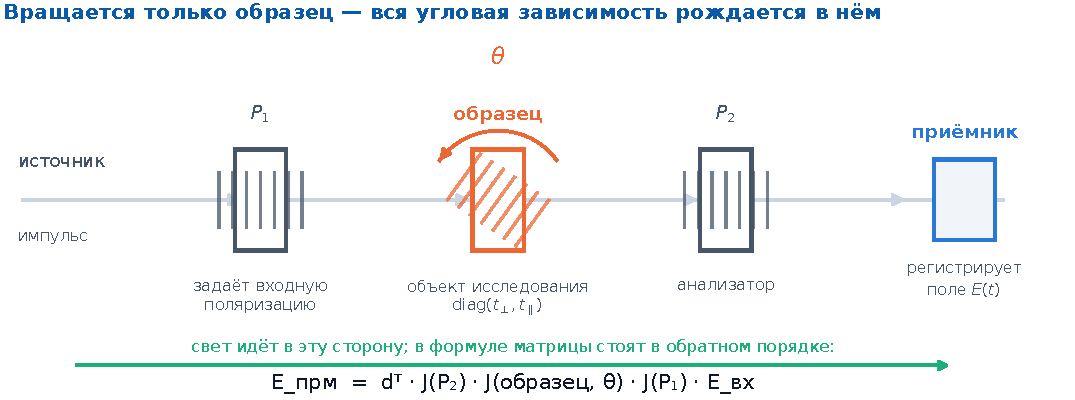
\includegraphics[width=\linewidth]{figures/fig01_cascade.pdf}
  \caption{Схема измерения на языке матриц Джонса; штриховка внутри элементов показывает
  направление проволок. Свет проходит элементы слева направо, а матрицы в формуле стоят в
  обратном порядке. Вращается только исследуемый образец; остальные элементы неподвижны, поэтому
  вся угловая зависимость наблюдаемой рождается в нём.}
  \label{fig:cascade}
\end{figure}

\begin{strict}[: вывод угловой зависимости]
Пусть вход поляризован вдоль~$x$, анализатор и приёмник тоже настроены на~$x$, а образец с
матрицей $\mathrm{diag}(\tperp,\tpar)$ повёрнут на~$\theta$. Подставляя~\eqref{eq:rotation} и
беря $x$-компоненту результата, получаем
\begin{equation}
  \Efield(\theta)=\tperp\cos^2\theta+\tpar\sin^2\theta .
  \label{eq:malus-jones}
\end{equation}
Это то самое выражение, которое в §\ref{sec:electrodynamics} было принято без вывода. При
$\tperp=1$, $\tpar=0$ оно даёт $\cos^2\theta$ по амплитуде, то есть $\cos^4\theta$ по энергии.
\end{strict}

\begin{intuition}[: как читать формулу~\eqref{eq:malus-jones}]
Два слагаемых~--- два пути, по которым поле попадает на приёмник. Первый: поле прошло через канал
пропускания образца, и его вклад ослаблен геометрической проекцией $\cos^2\theta$. Второй: поле
прошло через канал подавления, где образец обязан был его погасить, и вклад взвешен
$\sin^2\theta$. Вблизи $\theta=90^\circ$ первый путь закрыт геометрией, и на приёмник приходит
почти исключительно то, что \emph{просочилось}. Именно поэтому область глубокого подавления~---
самая информативная часть развёртки.
\end{intuition}

% ---------------------------------------------------------------------
\subsection{Реальный поляризатор: просачивание и его фаза}
\label{subsec:leakage}

Вынесем за скобку пропускание рабочего канала:
\begin{equation}
  \begin{pmatrix}\tperp&0\\0&\tpar\end{pmatrix}
  =\tperp\begin{pmatrix}1&0\\[2pt]0&\eta\,e^{\jj\delta}\end{pmatrix},
  \qquad
  \eta=\left|\frac{\tpar}{\tperp}\right|,
  \quad
  \delta=\arg\frac{\tpar}{\tperp}.
  \label{eq:leaky}
\end{equation}

Такая запись отделяет общий множитель (насколько прибор ослабляет свет вообще) от того, что нас
интересует: насколько плохо он подавляет ненужную поляризацию. Появились две содержательные
величины.

\begin{itemize}[leftmargin=1.4em,itemsep=0.35em]
  \item $\eta$~--- \term{просачивание}: доля \emph{амплитуды}, проходящая там, где должен быть
        ноль.
  \item $\delta$~--- \term{фаза просачивания}: насколько просочившееся поле запаздывает
        относительно прошедшего. В §\ref{sec:electrodynamics} мы видели, что линейная по частоте
        фаза есть временная задержка; поэтому осмысленная параметризация~---
        $\delta(\nu)=\delta_0+2\pi\nu\,\tleak$.
\end{itemize}

\begin{warning}[: амплитуда и мощность~--- не одно и то же]
\term{Коэффициент экстинкции} принято выражать через мощность:
\[
  \mathrm{ER}=\frac{1}{\eta^{2}},
  \qquad
  \mathrm{ER}\,[\text{дБ}]=-20\log_{10}\eta .
\]
Отсюда обычная ошибка на множитель два в децибелах: часть литературы (и, в частности,
аналитическая модель, к которой мы перейдём в §2) публикует коэффициенты \emph{по мощности}
$|\tperp|^2$ и $|\tpar|^2$, тогда как в матрицах Джонса стоят \emph{амплитудные}~$\tperp,\tpar$.
Забытый квадрат искажает результат ровно вдвое по шкале децибел.
\end{warning}

\begin{example}[: насколько хорош реальный поляризатор]\srckey{1.1}
На семи наборах измерений относительная амплитуда просачивания составила
\[
  \eta\approx0{,}012\ldots0{,}036,
\]
что отвечает коэффициенту экстинкции примерно от $29$ до $38$~дБ. Меньшие значения~--- у плотных
решёток, большие~--- у разреженных: связь с $D/P$ обсуждалась в §\ref{sec:electrodynamics}.

Для сравнения: плёночные поляризаторы, используемые в схеме как эталонные, дают лучше $39$~дБ~---
в терагерцовом диапазоне их можно считать идеальными проекторами.
\end{example}

\begin{figure}[t]
  \centering
  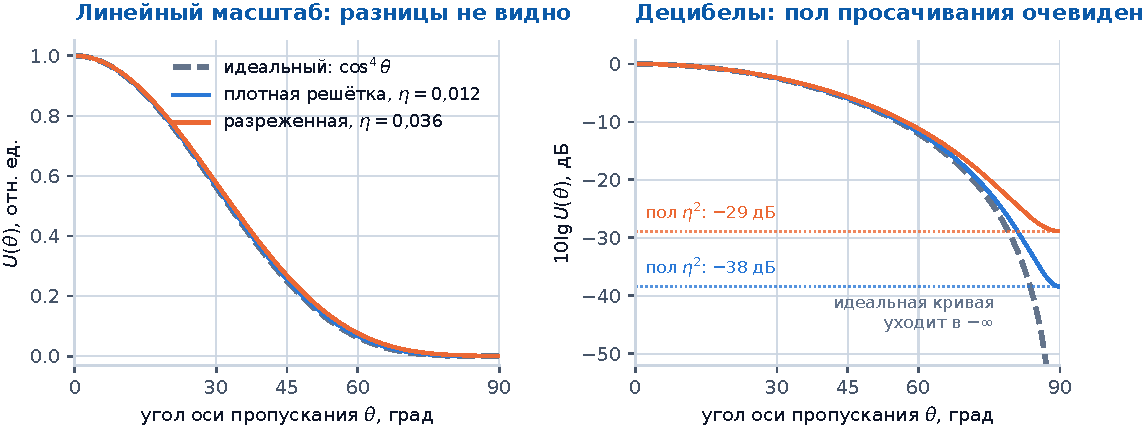
\includegraphics[width=\linewidth]{figures/fig01_malus_floor.pdf}
  \caption{Модельный расчёт по формуле~\eqref{eq:malus-jones} с реалистичными значениями
  просачивания. Слева, в линейном масштабе, идеальная и реальная кривые неразличимы. Справа, в
  децибелах, различие очевидно: вместо нуля при $90^\circ$ кривая упирается в \emph{пол}
  просачивания на уровне $\eta^2$. Уровень пола и есть измеряемая величина.}
  \label{fig:floor}
\end{figure}

\begin{intuition}[: почему просачивание видно только в логарифмическом масштабе]
Величина $\eta^2\sim10^{-3}$ на фоне единицы~--- одна тысячная. В линейном масштабе такая добавка
не видна глазом и почти не влияет на сумму квадратов невязок: подгонка её попросту не заметит.
В децибелах та же добавка~--- это разница между «минус бесконечность» и «минус тридцать»,
то есть между нулём и вполне уверенно измеримым сигналом.

Отсюда практическое правило, к которому мы вернёмся в §7 при обсуждении весов: \textbf{шкала, в
которой вы смотрите на данные, определяет, какие параметры вы способны измерить.}
\end{intuition}

% ---------------------------------------------------------------------
\subsection{Полная установка: где живут неидеальности}
\label{subsec:full-chain}

Запишем весь тракт. Свет проходит поляризатор~$P_1$, исследуемый образец под углом~$\theta$,
анализатор~$P_2$ и попадает на приёмник, чувствительный к одной линейной компоненте (вектор
чувствительности~$\mathbf{d}$):
\begin{equation}
  \Efield_{\text{прм}}
  =\mathbf{d}^{\mathsf T}\,\mathbf{J}_{P_2}\,\mathbf{J}_{\text{обр}}(\theta)\,
   \mathbf{J}_{P_1}\,\mathbf{E}_{\text{вх}} .
  \label{eq:chain}
\end{equation}

Идеализация~\eqref{eq:malus-jones} предполагала, что всё, кроме образца, идеально. В
действительности неидеален каждый сомножитель:

\begin{center}
\footnotesize
\setlength{\tabcolsep}{6pt}
\begin{tabular}{@{}p{0.17\linewidth}p{0.33\linewidth}>{\raggedright\arraybackslash}p{0.44\linewidth}@{}}
\toprule
\textbf{Элемент} & \textbf{Роль} & \textbf{Чем неидеален} \\
\midrule
$\mathbf{J}_{P_1}$ & задаёт входную поляризацию & собственное просачивание \\
$\mathbf{J}_{\text{обр}}(\theta)$ & \textbf{объект исследования} & здесь живут $\tperp$, $\tpar$
и через них~--- геометрия решётки \\
$\mathbf{J}_{P_2}$ & анализатор & собственное просачивание; ось может быть развёрнута
относительно приёмника \\
$\mathbf{d}$ & приёмник & чувствительность к «неправильной» компоненте (кросс-поляризация) \\
\bottomrule
\end{tabular}
\end{center}

\begin{warning}[: центральная методическая трудность всей задачи]
Малый сигнал, наблюдаемый в скрещённом положении, может родиться в трёх разных местах:
просачивание образца, просачивание анализатора, кросс-поляризация приёмника. \emph{По величине
сигнала на~$90^\circ$ они неразличимы принципиально}~--- складываются в одно число.

Различать их приходится по \term{угловой сигнатуре}: просачивание образца зависит от угла (входит
с весом $\sin^2\theta$), а аппаратные вклады от поворота образца не зависят вовсе. Это работает,
но лишь отчасти: сигнатуры недостаточно различны.
\end{warning}

\begin{example}[: насколько удалось разделить]\srckey{1.2}
Оценки просачивания образца и кросс-поляризации приёмника в совместной подгонке коррелируют с
коэффициентом~$0{,}73$. Разделение получено \emph{частичное}, и в выводах это указано как
ограничение метода, а не как результат.

Число $0{,}73$ стоит запомнить: в §5 мы научимся вычислять такие корреляции заранее, до
подгонки, из одного лишь плана эксперимента, а в §9~--- отличать «плохо разделено» от «не
разделено в принципе».
\end{example}

% ---------------------------------------------------------------------
\subsection{Усложнение, которое можно отвергнуть до вычислений}
\label{subsec:alignment}

Схема~\eqref{eq:chain} ставит естественный вопрос. Модель считает анализатор идеальным, а он
реален~--- у него своё просачивание. Не в нём ли причина того, что модель требует странно
малого эффективного диаметра (§\ref{sec:electrodynamics})? Соблазн очевиден: усложнить модель,
добавив второй реальный поляризатор, и посмотреть, что скажет подгонка.

Прежде чем усложнять, полезно посчитать на бумаге.

\begin{strict}[: теорема о выровненном анализаторе]
\emph{Если ось пропускания анализатора совпадает с осью чувствительности приёмника, то реальный
анализатор тождественно эквивалентен идеальному, умноженному на скаляр $t_{\perp,2}(\nu)$.}

\smallskip
\textbf{Доказательство.} Пусть обе оси направлены по~$x$, тогда $\mathbf{d}^{\mathsf T}=(1,0)$ и
\[
  \mathbf{d}^{\mathsf T}\mathbf{J}_{P_2}
  =(1,0)\begin{pmatrix}t_{\perp,2}&0\\[2pt]0&t_{\parallel,2}\end{pmatrix}
  =(t_{\perp,2},\,0)
  =t_{\perp,2}\,\mathbf{d}^{\mathsf T}.
\]
Вся информация о неидеальности анализатора содержится в $t_{\parallel,2}$, а он умножается на
нулевую компоненту вектора чувствительности и в наблюдаемую не входит. $\square$
\end{strict}

\begin{intuition}[: что именно доказано]
Неидеальность анализатора не «мала» и не «пренебрежима»~--- она \emph{ненаблюдаема}. Приёмник
физически не может отличить реальный выровненный анализатор от идеального: единственный след,
который остаётся,~--- общий множитель $t_{\perp,2}(\nu)$, одинаковый для всех углов.

А раз множитель не зависит от~$\theta$, он не способен изменить \emph{форму} угловой
зависимости. Все параметры, извлекаемые из формы~--- а это, в частности, эффективный диаметр,~---
обязаны остаться прежними.
\end{intuition}

\begin{example}[: предсказание, сделанное до расчёта, и его проверка]\srckey{1.3}
Из теоремы следовало конкретное численное предсказание: явное включение второго реального
поляризатора в модель не улучшит согласия с данными и не сдвинет оценку эффективного диаметра.
Проверка на измерениях:

\begin{itemize}[leftmargin=1.4em,itemsep=0.2em]
  \item изменение информационного критерия $\dAIC=+0{,}15$~--- усложнённая модель не лучше
        исходной (шкала $\Delta$AIC разбирается в §8; здесь достаточно знать, что это «ничего не
        изменилось»);
  \item оценка эффективного диаметра: $4{,}694$~мкм до усложнения и $4{,}694$~мкм после~---
        совпадение в четырёх значащих цифрах.
\end{itemize}

Модель усложнили честно, и она отказалась усложняться ровно так, как было предсказано на бумаге.
\end{example}

\begin{tcolorbox}[enhanced,colback=cS1!7,colframe=cS1,boxrule=0pt,leftrule=3pt,arc=1pt]
\textbf{Мораль для метода.} Прежде чем усложнять модель и запускать подгонку, проверьте, не
сводится ли усложнение к общему множителю, не зависящему от переменной, по которой идёт
развёртка. Если сводится~--- подгонка заведомо ничего не покажет, и это известно заранее и
бесплатно. Такие «теоремы редукции» экономят недели вычислений и, что важнее, избавляют от
соблазна истолковать шум как эффект.
\end{tcolorbox}

\begin{warning}[: условие теоремы существенно]
Требуется именно \emph{выравнивание} осей анализатора и приёмника. Если они развёрнуты на
угол~$\phi_2$, произведение $\mathbf{d}^{\mathsf T}\mathbf{J}_{P_2}$ перестаёт быть
пропорциональным $\mathbf{d}^{\mathsf T}$, просачивание анализатора становится наблюдаемым и
подмешивается к просачиванию образца. Теорема~--- не разрешение не думать об анализаторе, а
указание, что именно нужно контролировать в юстировке.
\end{warning}

% ---------------------------------------------------------------------
\subsection{Границы применимости формализма}
\label{subsec:limits}

\begin{strict}
Матрицы Джонса описывают \textbf{полностью поляризованный когерентный} свет. Для частично
поляризованного или частично когерентного излучения двух комплексных амплитуд недостаточно:
нужен более общий аппарат~--- вектор Стокса и матрицы Мюллера ($4\times4$, действуют на
интенсивности, а не на поля).
\end{strict}

\noindent
В нашем случае формализм Джонса законен, и по вполне конкретной причине: приёмник регистрирует
поле когерентно (§\ref{sec:electrodynamics}), то есть измеряет амплитуду и фазу, а не усреднённую
мощность. Это то же самое свойство установки, из-за которого угловая зависимость содержит пять
независимых чисел, а не три.

\begin{intuition}[: связь двух утверждений]
Одно физическое обстоятельство~--- когерентная регистрация поля~--- даёт сразу две вещи:
законность матриц Джонса и наличие перекрёстного члена в наблюдаемой. Если бы приёмник мерил
интенсивность, пришлось бы перейти к матрицам Мюллера, и вместе с фазой исчезла бы часть
информации~--- в частности, задержка просачивания.
\end{intuition}

% ---------------------------------------------------------------------
\subsection{Типичные ошибки этого параграфа}

\begin{enumerate}[leftmargin=1.6em,itemsep=0.25em]
  \item Переставить сомножители в каскаде. Свет идёт слева направо, матрицы перемножаются справа
        налево: $\mathbf{J}_2\mathbf{J}_1\neq\mathbf{J}_1\mathbf{J}_2$.
  \item Ожидать $\cos^2\theta$ вместо $\cos^4\theta$. В схеме с анализатором проекция происходит
        дважды (§\ref{subsec:malus}).
  \item Спутать амплитудные коэффициенты с коэффициентами по мощности. Множитель два в
        децибелах~--- самая живучая ошибка в этой области.
  \item Отождествить просачивание и коэффициент экстинкции: $\mathrm{ER}=1/\eta^2$, это разные
        величины и разные шкалы.
  \item Отбросить фазу коэффициентов, оставив модули. Вместе с фазой теряется задержка
        просачивания~--- ровно то, ради чего ставился когерентный эксперимент.
  \item Применить матрицы Джонса к частично поляризованному свету (§\ref{subsec:limits}).
  \item Считать, что малый сигнал в скрещённом положении заведомо принадлежит образцу. У него
        три возможных источника, и разделяются они только по угловой зависимости
        (§\ref{subsec:full-chain}).
\end{enumerate}

\clearpage
